直線とカーブ両方あり,周期境界条件を持ち複数の対面走行できるように,
楕円コースで実験する.
コースの中(青い部分)にロボットをランダムに配置し,半数のロボットが右回り
($b_{\rm L}>b_{\rm R}$),
残りのロボットが左回り($b_{\rm L}<b_{\rm R}$)の向きで,
速度0からほぼ同時にスタート,約8分間実験する.

ロボットがtof距離センサーでコースの障害物までの距離を測って,
非線形感覚運動写像モデルにより走行する.

コースの青い部分の中央(図\ref{fig:cource}黒い線)でコースの長さを測る,
コースの長さ($L$)は7.32$m$,今回ロボットの台数($N$)は8台である.
ロボットの線密度 $ \rho = \frac{N}{L} = 1.09 ({\rm 台/m})$である.

両側の壁を移動させて,コースの幅($w$)を
$43cm$,$49.5cm$,$56cm$,$62.5cm$,$69cm$へ変化させ,実験する.


\begin{figure}[h]
    \begin{minipage}{0.48\linewidth}
        \centering
        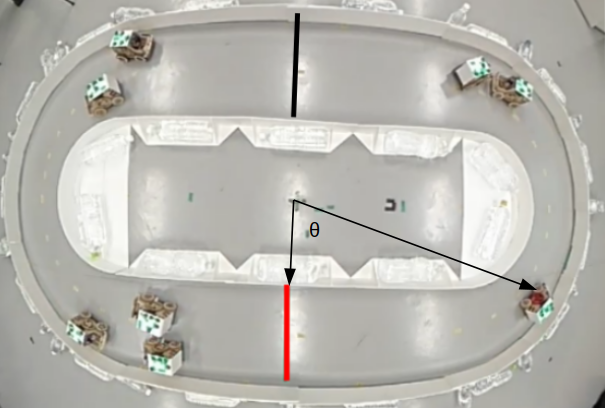
\includegraphics[width=0.9\linewidth]{course3.jpg}
        \caption{実験の様子と$\theta$の説明}
        \label{course1}
    \end{minipage}
    \begin{minipage}{0.48\linewidth}
        \centering
        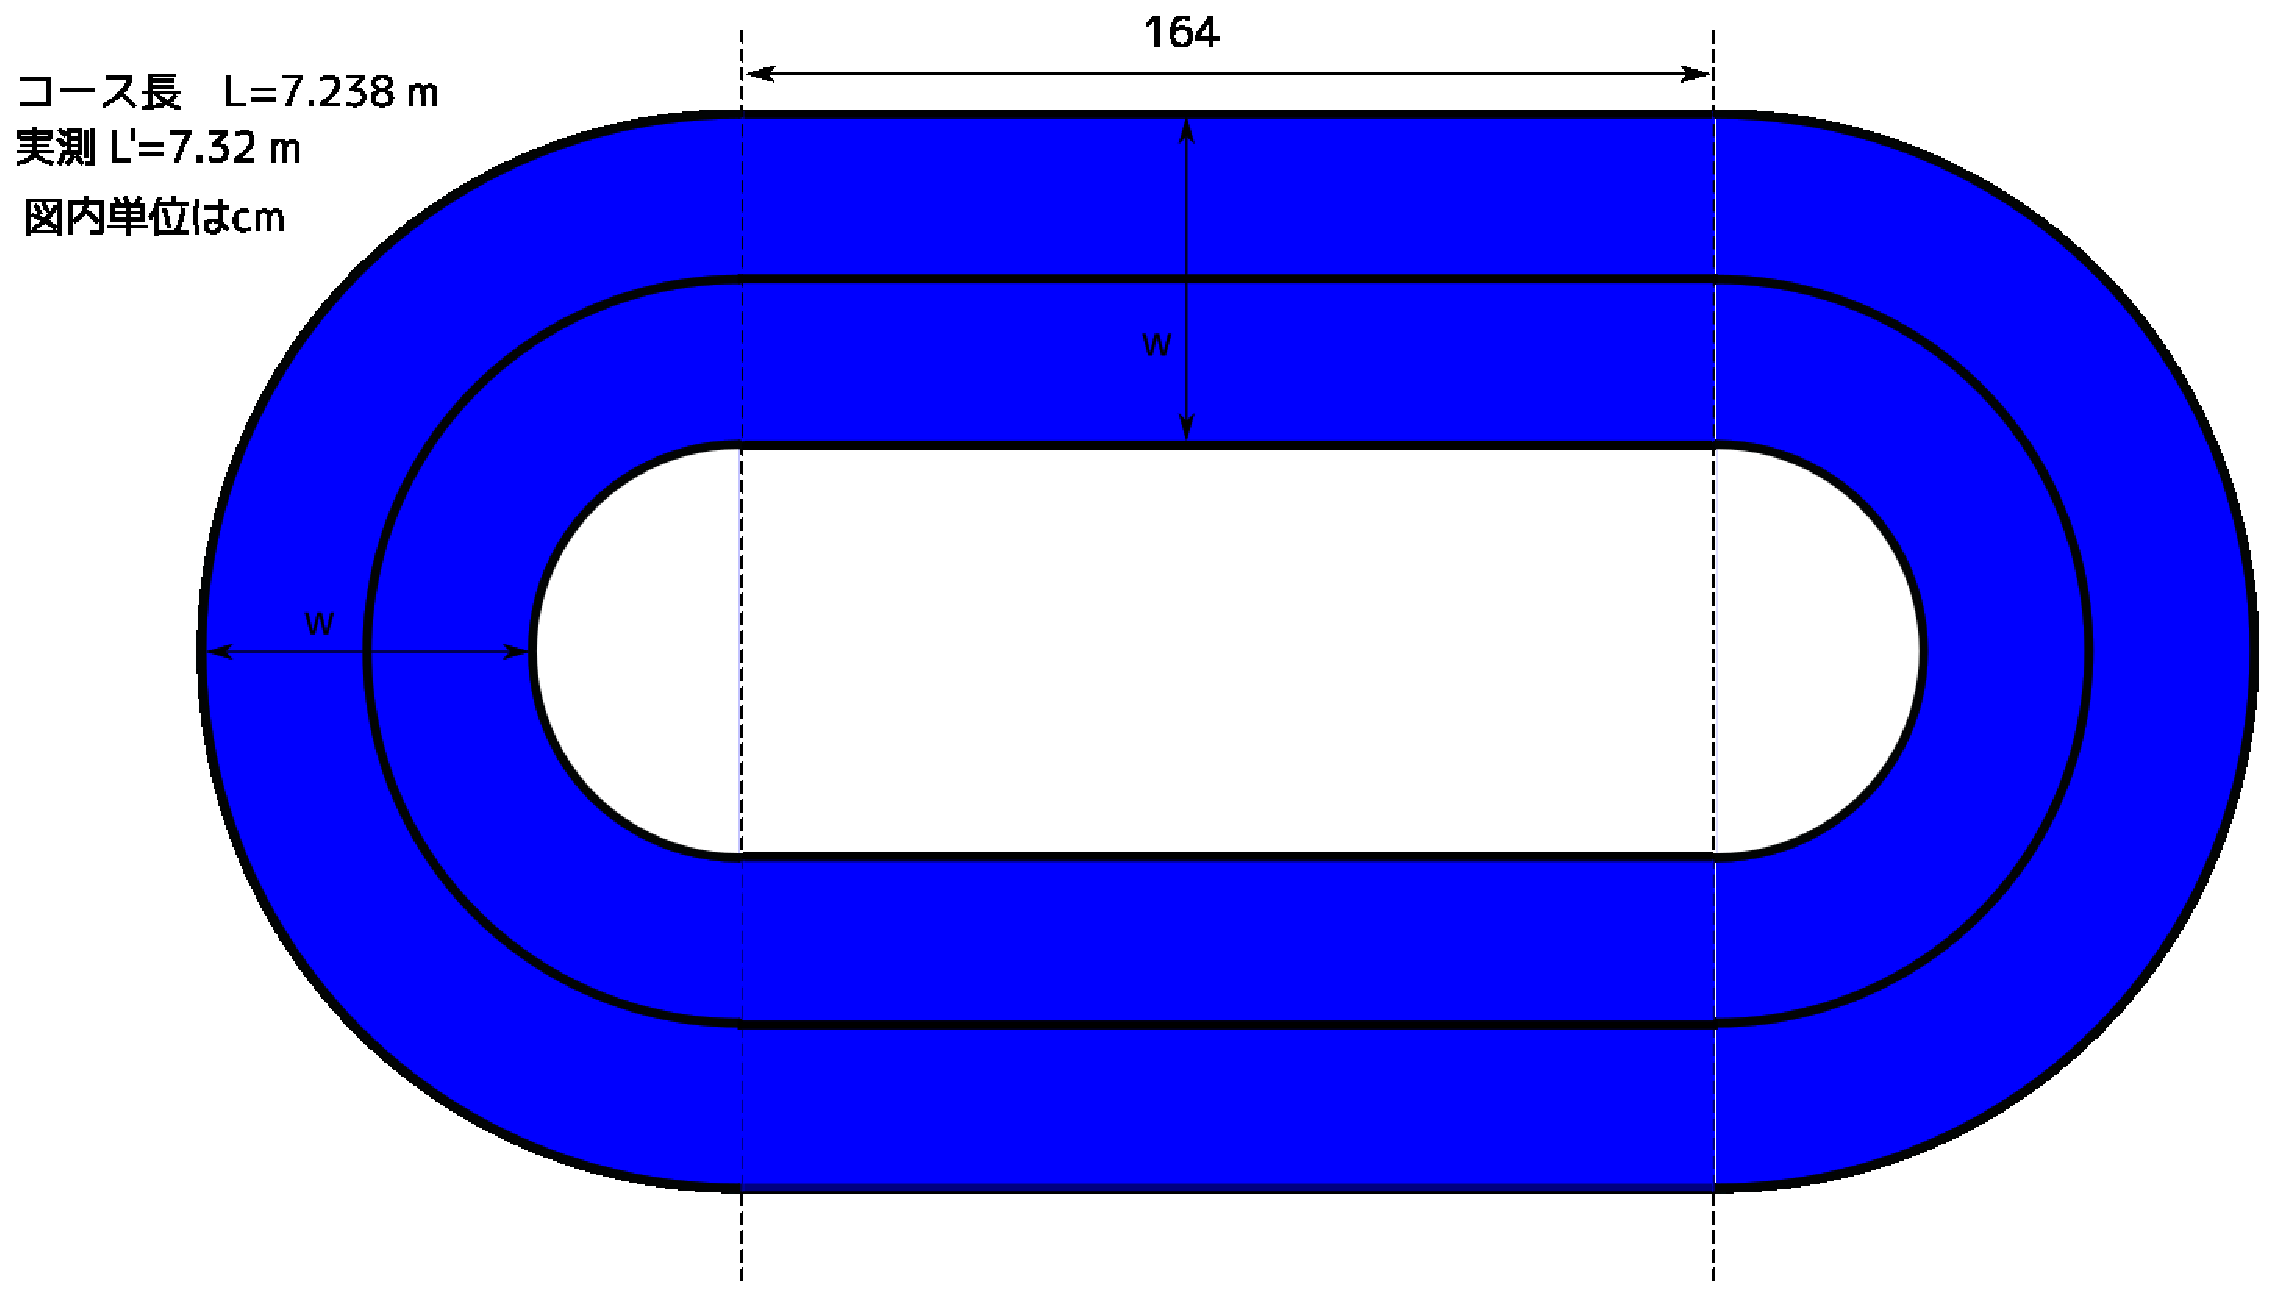
\includegraphics[width=1.0\linewidth]{Oval_h2.eps}
        \caption{\label{fig:cource}コースレイアウト}
        \label{course2}
    \end{minipage}
\end{figure}



図\ref{course1}の赤い線を計測ラインとして,ロボットが左から右へ線を通過したら流量+1,
右から左へ線を通過したら流量-1とする.
図\ref{course2}の横軸が時間(秒),縦軸がコース中心からみたロボットの位置角度
$\theta$(図\ref{course1}),ロボットが赤い線から反時計回りで黒い線まで,
$\theta$が0から$\pi$に変わる.
赤い線から時計回りで黒い線まで,$\theta$が0から$-\pi$に変わる.
計測ライン(赤い線)を通過して,台数($n$)を計測する.
$T_{\rm 1d}$はone direction flow 状態になる時間(分),$w$がコースの幅(単位:$m$),
流量$Q_i$を式(\ref{eq:flow})で,その平均値を式(\ref{eq:flow_ave})で計算する.

\begin{eqnarray}
Q_i &=& \frac{|n_i|}{wT_{\rm 1d}}
\label{eq:flow} \\
\bar{Q} &=& \frac{1}{N_{\rm exp}}\sum_{i=1}^{N_{\rm exp}} Q_i
\label{eq:flow_ave} 
\end{eqnarray}
$i$は実験回数を,また$N_{\rm exp}$は全実験回数を表す.
